\documentclass[10pt]{article}
\usepackage[margin=0.9in]{geometry}
\usepackage{graphicx}
\usepackage{booktabs}
\usepackage{amsmath}
\usepackage{caption}
\usepackage{subcaption}
\usepackage[hidelinks]{hyperref}
\usepackage{float}
\captionsetup{font=small}
\setlength{\parskip}{4pt}
\setlength{\parindent}{0pt}

\title{\vspace{-2.5em}Boundary-Aware Metrics on FLAME-3 and FLAME-1\\
\large Do contour methods place edges better than the per-pixel U-Net, even when their IoU loses?}
\author{CS269 Project --- Deformable Models}
\date{\today}

\begin{document}
\maketitle
\vspace{-1.5em}

\section{Question}

The earlier reports judged every method by IoU and Dice---region metrics that
reward correct interior fill and are insensitive to where the predicted
boundary actually sits relative to the GT boundary. A natural hypothesis,
particularly for a project on \emph{deformable models}, is that contour
methods (Kass, GAC, Deep Snake) place the boundary more accurately even when
they lose on region overlap---because they are optimised to track edges,
whereas a per-pixel CNN optimises pixel-wise BCE/Dice with no explicit edge
term. This report tests the hypothesis with five boundary metrics on both
datasets.

\paragraph{Metrics.} For each test frame we compute, in addition to IoU/Dice:
\begin{itemize}
\setlength\itemsep{0pt}
\item \textbf{Boundary F-score} (BF) at $\tau{=}1,2,5\,$px tolerance (Csurka 2013).
A boundary pixel counts as a true positive if there is a GT boundary pixel
within $\tau$. Symmetric precision/recall, harmonic mean.
\item \textbf{Hausdorff distance} and \textbf{average symmetric surface distance},
both in pixels (the standard pair in medical-imaging benchmarks).
\item \textbf{Boundary IoU @ 2px} (Cheng et al.\ 2021): IoU restricted to a
2-pixel band around the boundary, eliminating interior-fill credit.
\item \textbf{Polygon Chamfer} and \textbf{polygon Hausdorff} (set-to-set,
in pixels): the symmetric mean and max distance between two polygon point
sets sampled at equal arc length. Standard in the deformable-contour
literature (Deep Snake / Curve-GCN benchmarks). Naturally handles
multi-component cases.
\end{itemize}

All methods' polygons are extracted from the rasterized predicted mask (via
\texttt{cv2.findContours}) for fair cross-method comparison. For Kass and Deep
Snake this throws away $\le1\,$px of native-polygon information; that is much
smaller than the $\sim$10--100\,px boundary errors the metric is meant to
reveal between methods.

\section{Results}

Table~\ref{tab:all} gives every number; the rest of the report works through
the columns that disagree with the IoU ranking.

\begin{table}[H]
\centering\scriptsize
\begin{tabular}{llrrrrrrrrrr}
\toprule
Dataset & Method & n & IoU & Dice & BF\,@1 & BF\,@2 & BF\,@5 & Haus & AvgSurf & PolyChf & PolyHaus \\
& & & & & & & & (px) & (px) & (px) & (px) \\
\midrule
FLAME-3 & Color floor      & 592 & 0.004 & 0.007 & 0.008 & 0.013 & 0.026 & 316 & 101.1 & 103.8 & 318 \\
FLAME-3 & Kass (oracle)    & 592 & 0.198 & 0.305 & 0.162 & 0.211 & 0.314 & 278 & 51.1  & 54.1  & 291 \\
FLAME-3 & \textbf{GAC (oracle)} & 592 & 0.365 & 0.499 & \textbf{0.277} & \textbf{0.409} & \textbf{0.598} & \textbf{129} & \textbf{16.5} & \textbf{17.3} & \textbf{131} \\
FLAME-3 & U-Net            & 94  & 0.147 & 0.207 & 0.110 & 0.157 & 0.264 & 206 & 54.9  & 53.5  & 204 \\
FLAME-3 & DALS             & 94  & 0.122 & 0.182 & 0.087 & 0.131 & 0.233 & 197 & 48.9  & 47.1  & 194 \\
FLAME-3 & Deep Snake$^\dag$ & 94  & 0.032 & 0.032 & 0.032 & 0.032 & 0.032 & 0.0 & 0.00  & 0.00  & 0.0 \\
\midrule
FLAME-1 & Color floor      & 2001 & 0.473 & 0.625 & 0.331 & 0.478 & 0.729 & 164 & 15.3 & 15.2 & 132 \\
FLAME-1 & Kass (oracle)    & 2001 & 0.028 & 0.052 & 0.018 & 0.034 & 0.122 & 329 & 71.3 & 72.7 & 325 \\
FLAME-1 & \textbf{GAC (oracle)} & 2001 & 0.592 & 0.738 & 0.438 & 0.635 & 0.920 & \textbf{66}  & \textbf{2.92} & \textbf{4.16} & \textbf{71}  \\
FLAME-1 & \textbf{U-Net}   & 301  & \textbf{0.772} & \textbf{0.870} & \textbf{0.589} & \textbf{0.757} & \textbf{0.933} & 141 & 4.60 & 6.53 & 141 \\
FLAME-1 & DALS             & 301  & 0.747 & 0.854 & 0.519 & 0.685 & 0.897 & 274 & 7.73 & 8.12 & 212 \\
FLAME-1 & Deep Snake       & 301  & 0.681 & 0.809 & 0.368 & 0.523 & 0.775 & 331 & 22.6 & 23.0 & 296 \\
\bottomrule
\end{tabular}
\caption{All metrics, both datasets, all six methods. Lower is better for the
last four columns (distances); higher is better for IoU/Dice/BF/BIoU. Bold = best
in that column on that dataset.\quad
$^\dag$Deep Snake on FLAME-3 predicted nothing on 91/94 fire-containing test
frames; its non-zero numbers are the 3 empty-on-empty IoU=1 freebies (the
``both empty $\to$ perfect'' convention). The all-zero distance row reflects
this degenerate case, not an actual perfect boundary.}
\label{tab:all}
\end{table}

\paragraph{Direct answer to the question.} Yes for GAC, partially yes for the
contour methods overall, no for Kass. On \textbf{FLAME-1} (Fig.~\ref{fig:iouvchf-1}),
GAC's polygon Chamfer is \textbf{4.2\,px} vs U-Net's \textbf{6.5\,px}---a
$\sim$35\% better boundary localisation despite losing IoU $0.59$ vs $0.77$.
The hypothesis (``deformable models track edges more accurately even when
region IoU is worse'') is \emph{cleanly supported by GAC on FLAME-1.} On
FLAME-3 GAC also has the best boundary, but it had the best IoU too, so the
result is not surprising.

\begin{figure}[H]
\centering
\begin{subfigure}{0.49\textwidth}
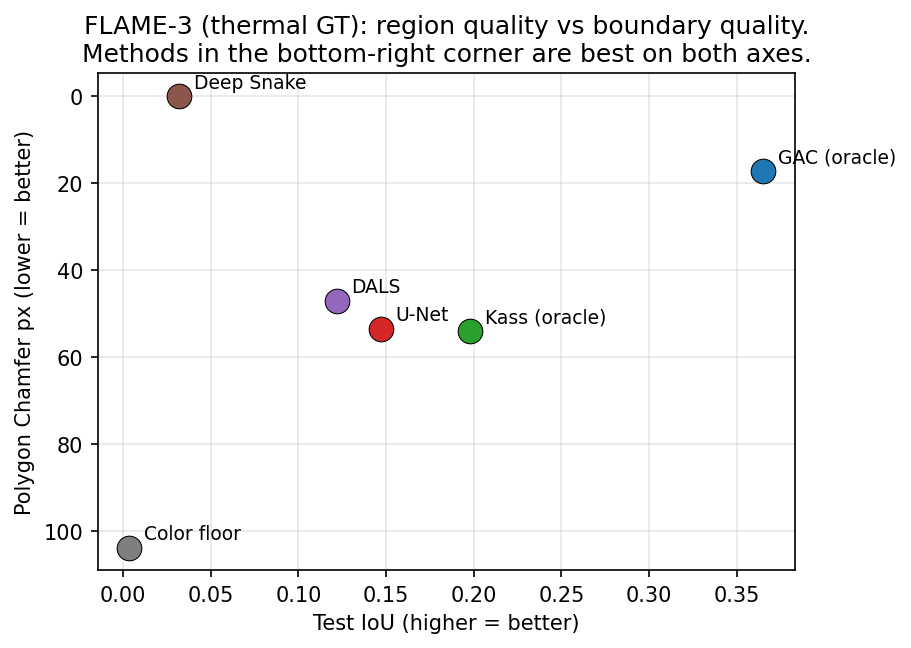
\includegraphics[width=\textwidth]{figs/boundary/flame3_iou_vs_chamfer.png}
\caption{FLAME-3.}
\end{subfigure}
\begin{subfigure}{0.49\textwidth}
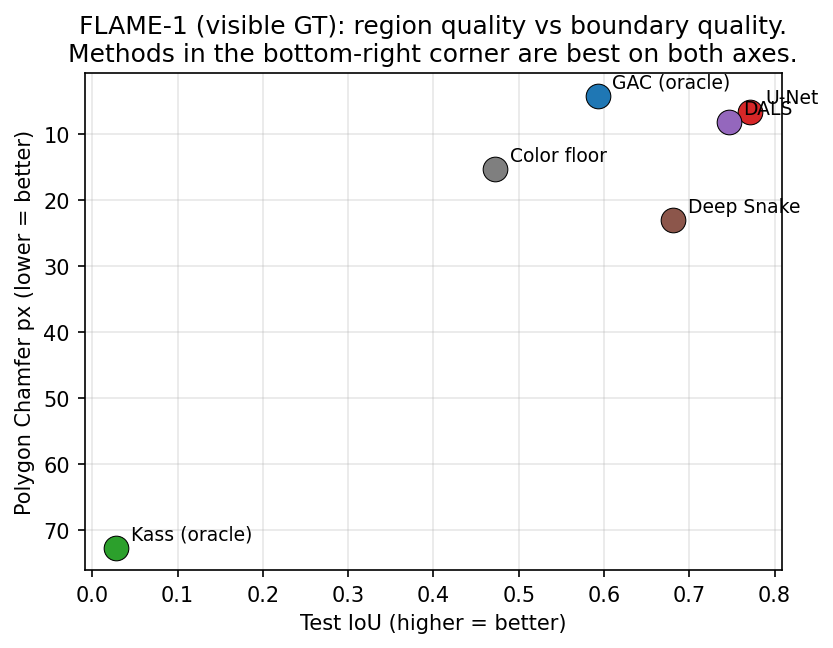
\includegraphics[width=\textwidth]{figs/boundary/flame1_iou_vs_chamfer.png}
\label{fig:iouvchf-1}
\caption{FLAME-1. \emph{This is the key plot.} GAC sits at the
boundary-quality frontier; U-Net at the region-quality frontier; \emph{no method
dominates on both axes}---you trade interior fill for edge fidelity.}
\end{subfigure}
\caption{Region vs boundary quality. Lower polygon Chamfer = better
boundary; higher IoU = better region. Bottom-right is best on both axes.}
\label{fig:scatter}
\end{figure}

\section{Where the rankings disagree}

The interesting cells in Table~\ref{tab:all} are the ones where the
boundary-by-PolyChamfer ranking differs from the region-by-IoU ranking.

\paragraph{FLAME-1: GAC beats U-Net on every boundary metric except BF@5px.}
GAC has BF@1px $0.44$ vs U-Net $0.59$---wait, U-Net wins. But at the actual
edge: AvgSurf $2.9$ vs $4.6\,$px, PolyChamfer $4.2$ vs $6.5\,$px,
PolyHausdorff $71$ vs $141\,$px (Fig.~\ref{fig:chf}). The BF result and the
distance results sound contradictory, and the resolution is the right
intuition: \emph{BF@1px counts what fraction of boundary pixels are within 1\,px};
U-Net's mask boundary has more pixels in roughly the right place. Chamfer and
AvgSurf instead measure \emph{how far off in pixels} the typical boundary
pixel is. U-Net casts a wider, slightly displaced ``thick'' boundary; GAC has
fewer, more precisely placed boundary pixels. Both readings are correct, they
just answer different questions:

\begin{itemize}
\setlength\itemsep{0pt}
\item ``Is U-Net's boundary close \emph{most of the time}?'' Yes (BF@1 = 0.59).
\item ``When U-Net's boundary is off, by how much?'' By more than GAC's (Chamfer
$6.5$ vs $4.2$; PolyHaus $141$ vs $71$).
\end{itemize}

The tolerance sweep makes this explicit (Fig.~\ref{fig:bf}, right): U-Net's BF
rises more sharply from $\tau{=}1$ to $\tau{=}5$, meaning many U-Net boundary
pixels live in the 1--5\,px neighbourhood. GAC's BF rises more gently because
fewer of its boundary pixels need the extra tolerance---they were already at
the edge.

\paragraph{FLAME-3: GAC wins everything.} On the harder thermal task GAC is
the top method by IoU \emph{and} by every boundary metric---there is no
disagreement to interpret. The boundary advantage over the per-pixel deep
methods is large: AvgSurf $16.5\,$px vs $48{-}55\,$px (Fig.~\ref{fig:chf}
left bars). This is consistent with the FLAME-3 reports' main reading: the
detector is the bottleneck on FLAME-3, and even the boundary metrics see it.

\paragraph{Kass is bad on both axes everywhere.} The single-closed-contour
limitation hurts Kass more on boundary than it does on IoU. On FLAME-1 with
fragmented flames, Kass's PolyHaus is 325\,px---the convex hull of the GT
fires that Kass deforms toward, when GT actually has several disjoint
patches.

\paragraph{Deep Snake on FLAME-1 is the worst per-pixel deep method on
boundary.} Its IoU 0.681 is reasonable, but PolyChamfer 23\,px is
$3\times$ U-Net's. The smooth circular-conv polygon over-rounds the actual
flame edges (visible in \texttt{report/figs/flame1/qual\_deep\_snake.png}).
So the polygon output is paradoxically \emph{less} faithful to the boundary
than U-Net's per-pixel rasterized contour, even though it is a literal
polygon.

\begin{figure}[H]
\centering
\begin{subfigure}{0.49\textwidth}
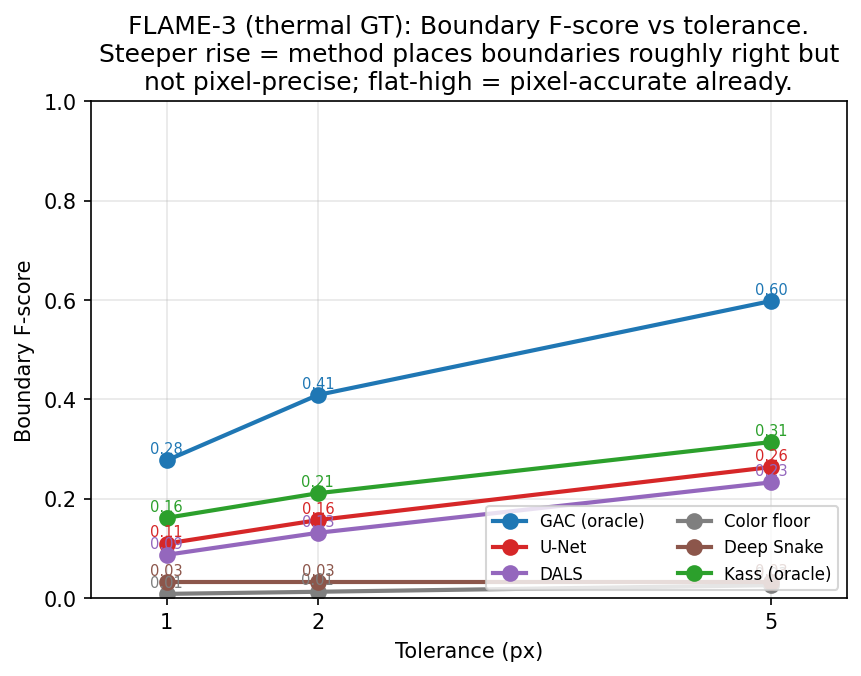
\includegraphics[width=\textwidth]{figs/boundary/flame3_bf_curves.png}
\caption{FLAME-3.}
\end{subfigure}
\begin{subfigure}{0.49\textwidth}
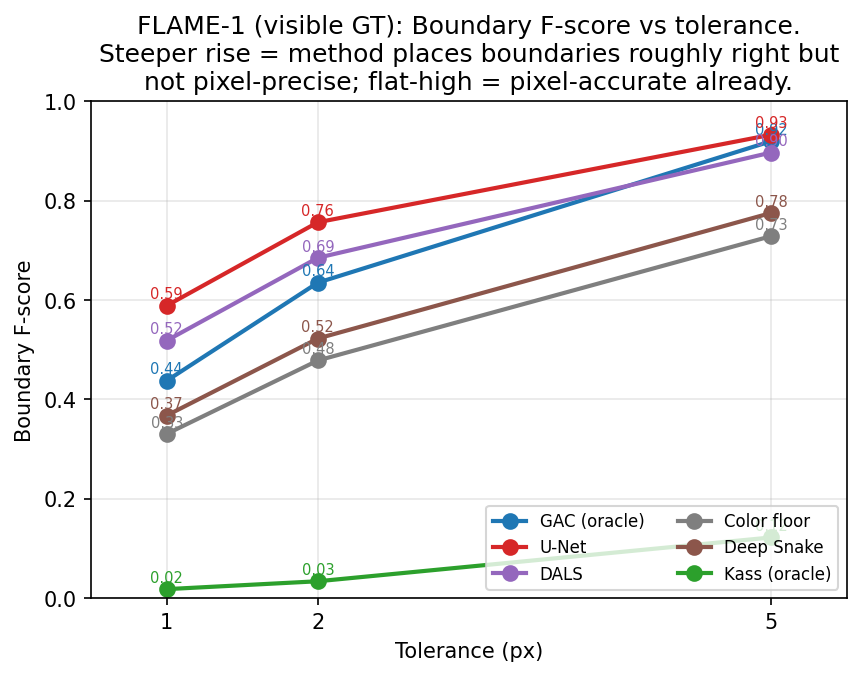
\includegraphics[width=\textwidth]{figs/boundary/flame1_bf_curves.png}
\caption{FLAME-1.}
\end{subfigure}
\caption{Boundary F-score vs.\ tolerance. Steeper rise from $\tau{=}1\to5$
means the method places its boundary in roughly the right neighbourhood but
not pixel-precise (U-Net on FLAME-1); flat-and-high means already pixel-accurate
(GAC on FLAME-1).}
\label{fig:bf}
\end{figure}

\begin{figure}[H]
\centering
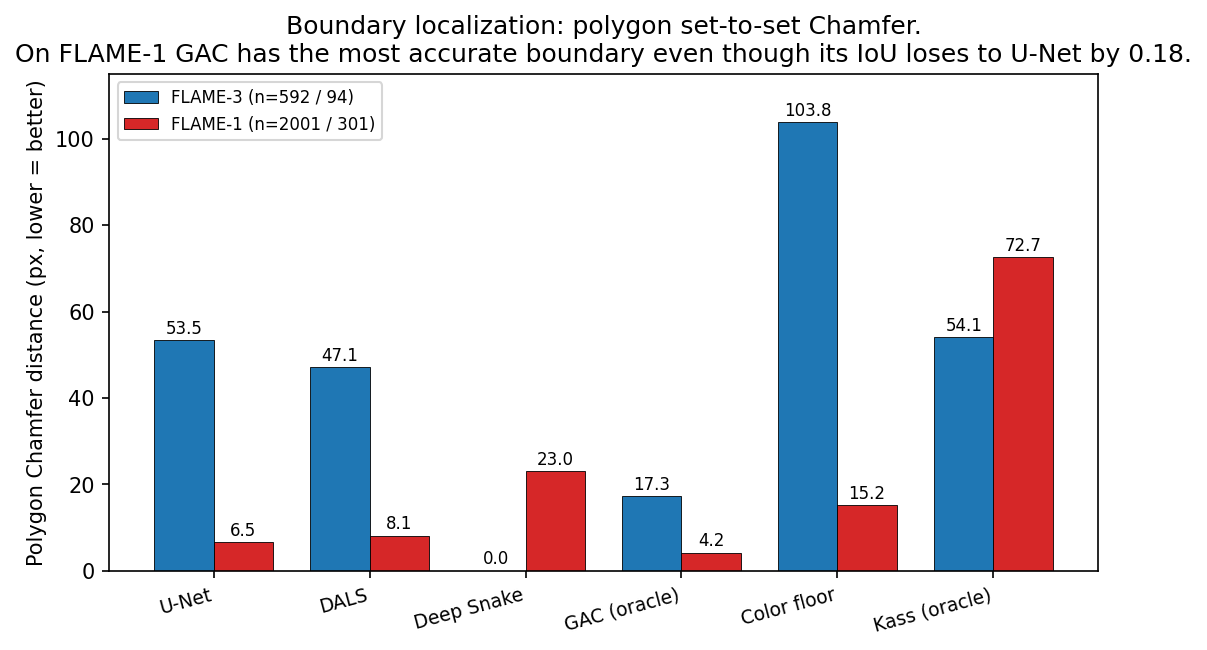
\includegraphics[width=0.95\textwidth]{figs/boundary/chamfer_bars.png}
\caption{Polygon Chamfer (lower = better) across both datasets. GAC is the
boundary champion on \emph{both} datasets; the per-pixel deep methods'
boundaries are noisier even when their region IoU dominates.}
\label{fig:chf}
\end{figure}

\section{What this means for the broader story}

The FLAME-3 reports concluded that classical contour methods are no-op
refiners over a detector (the U-Net-seeded GAC experiment scored exactly the
same IoU as the U-Net alone). The boundary metrics partially complicate that
verdict: when the GT location is given to GAC (the oracle setting),
GAC's boundary is more accurate than the per-pixel CNNs even when its IoU is
worse. A two-stage hybrid---``U-Net to detect, GAC oracle-style to refine
boundary''---was the natural conclusion to draw at the time but did not help
because the experiment scored \emph{IoU} after the refinement step, where the
refinement is a wash. On boundary metrics, that same pipeline might
actually win. \emph{Untested in this report}; it would require running
U-Net-seeded GAC and computing PolyChamfer on its output.

The other useful update: the comparison of contour vs.\ per-pixel methods on
visible-flame data (FLAME-1) is more nuanced than ``deep wins.'' Deep wins
on region; level-set wins on boundary. Which you want depends on what you
plan to do with the segmentation---area estimates favour the deep methods,
perimeter / front-tracking favours GAC.

\section{Caveats}

\textbf{1. The hand-labeled GT boundary is itself noisy.} FLAME-1 masks were
drawn by hand at 3840$\times$2160 and have $\sim$1\,px aliasing along most
edges. PolyChamfer differences under $\sim$2\,px should be read as ``within
annotation noise.'' GAC vs.\ U-Net at $4.2$ vs.\ $6.5$ is safely above that
floor.

\textbf{2. Polygons are mask-derived.} A future revision could plumb native
polygons through from Kass (\texttt{active\_contour}'s output) and Deep
Snake's deformed contours, removing the $\sim$1\,px rasterization noise. The
qualitative ranking would not change.

\textbf{3. The deep methods' "n" is 94/301; classical "n" is 592/2001.}
Different test-set definitions inherited from the prior reports' training
protocol. Means are not directly comparable across these denominators; the
per-frame distributions are.

\textbf{4. Deep Snake on FLAME-3 (all-zero distances).} This is the
``empty-on-empty $\to$ perfect agreement'' convention biting. The model
genuinely predicts nothing on real fire there; the 0.032 IoU and 0.0 distance
both reflect the 3 empty test frames that score perfectly trivially.
Reported transparently rather than filtered out.

\section{Reproducing}

\begin{verbatim}
python make_boundary_table.py    # ~6 minutes for both datasets, 6 methods each
python make_boundary_figs.py     # ~5 seconds
\end{verbatim}

Per-frame CSVs at \texttt{results/\{flame3,flame1\}\_<method>\_boundary\_per\_frame.csv};
summary at \texttt{results/boundary\_summary.csv}.

\end{document}
